  
\documentclass[11pt, letterpaper]{article}
\usepackage[letterpaper, portrait, margin=1in]{geometry}

\usepackage{amsmath,amsfonts,amsthm} % Math packages
\usepackage{fancyhdr}
\usepackage{datetime}
\usepackage{enumitem}
\usepackage{titlesec}
\usepackage{graphicx}
\usepackage[none]{hyphenat}

\usepackage{bera}

\fancyhf{}
%\fancyhead[L]{Associated Students of Walla Walla University}
\fancyhead[R]{Constitution}
\fancyfoot[L]{\fontsize{7}{12} \selectfont Last compiled: \today\ \currenttime}
\fancyfoot[C,CO]{Page \thepage}
\pagestyle{fancy}
\fancyhead[L]{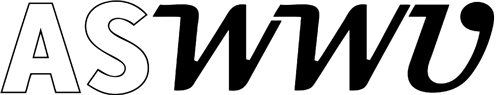
\includegraphics[scale=0.2]{LogoCrop_BLACK_500px.png}}

\usepackage{lineno, blindtext, color}
\linenumbers
\renewcommand\thelinenumber{\color{red}\arabic{linenumber}}

\def\changemargin#1#2{\list{}{\rightmargin#2\leftmargin#1}\item[]}
\let\endchangemargin=\endlist 

%\renewcommand{\thesection}{\arabic{section} \hspace{1mm} Article \Roman{section}.\hspace{-5mm}}
%\renewcommand{\thesubsection}{\hspace{1cm}\arabic{section}.\arabic{subsection}. Section %\arabic{subsection}. \hspace{-5mm}}

%\renewcommand\thesection{\Roman{section}} 
%\renewcommand\thesubsection{\thesection.\Roman{subsection}} 
%\titleformat{\section}[block]{\bfseries}{\thesection.}{1em}{} 
%\titleformat{\subsection}[block]{\hspace{2em}}{\thesubsection}{1em}{}

%\titleformat{\subsection}[display]{\normalfont}{\thesubsection}{1ex}{test}[test]

\usepackage{parskip}

\makeatletter

%%%%%%%%%%%%%%%%%%%%%%%%%%%%%%%%%%%
% Configuration
\def\sectionindent{10mm}
\def\subsectionindent{12mm}
\def\subsubsectionindent{14mm}

%%%%%%%%%%%%%%%%%%%%%%%%%%%%%%%%%%%
% Some derived quantities
% (you should manually update these)

\def\subsectiontotalindent{22mm} 
% = \sectionindent + \subsectionindent

\def\subsubsectiontotalindent{36mm}
% = \sectionindent + \subsectionindent + \subsubsectionindent

%%%%%%%%%%%%%%%%%%%%%%%%%%%%%%%%%%%%%%%%%%
% The following code is adapted from some sample code by 
% Vincent Zoonekynd, made available at the following website:
% http://zoonek.free.fr/LaTeX/LaTeX_samples_section/0.html 

%%%%%%%%%%%%%%%%%%%%%%%%%%%%%%%%%%%%%%%%%%
% Redefining \section and \section*

\def\article{\@ifstar\unnumberedsection\numberedsection}
\def\numberedsection{\@ifnextchar[%]
  \numberedsectionwithtwoarguments\numberedsectionwithoneargument}
\def\unnumberedsection{\@ifnextchar[%]
  \unnumberedsectionwithtwoarguments\unnumberedsectionwithoneargument}
\def\numberedsectionwithoneargument#1{\numberedsectionwithtwoarguments[#1]{#1}}
\def\unnumberedsectionwithoneargument#1{\unnumberedsectionwithtwoarguments[#1]{#1}}
\def\numberedsectionwithtwoarguments[#1]#2{%
  \ifhmode\par\fi
  \removelastskip
  \vskip 1ex\goodbreak
  \refstepcounter{section}%
  \noindent
  \begingroup
  \leavevmode\Large\bfseries\raggedright
  \rlap{\thesection}%
  \hspace{\sectionindent} Article \Roman{section}. \hspace{0.1mm} %
  #2
  \par
  \endgroup
  \vskip -1ex\nobreak
  \addcontentsline{toc}{section}{%
    \protect\numberline{\thesection}%
    #1}%
  \leftskip=\sectionindent\relax%
  }
\def\unnumberedsectionwithtwoarguments[#1]#2{%
  \ifhmode\par\fi
  \removelastskip
  \vskip 3ex\goodbreak
%  \refstepcounter{section}%
  \noindent
  \begingroup
  \leavevmode\Large\bfseries\raggedright
  %\rlap{\thesection}%
  \hspace{\sectionindent}%
  #2
  \par
  \endgroup
  \vskip 2ex\nobreak
  \addcontentsline{toc}{section}{%
%    \protect\numberline{\thesection}%
    #1}%
  \leftskip=\sectionindent\relax%
}

%%%%%%%%%%%%%%%%%%%%%%%%%%%%%%%%%%%%%%%%%%
% Redefining \subsection and \subsection*
%%%%%%%%%%%%%%%%%%%%%%%%%%%%%%%%%%%%%%%%%%

\def\section{\@ifstar\unnumberedsubsection\numberedsubsection}
\def\numberedsubsection{\@ifnextchar[%]
  \numberedsubsectionwithtwoarguments\numberedsubsectionwithoneargument}
\def\unnumberedsubsection{\@ifnextchar[%]
  \unnumberedsubsectionwithtwoarguments\unnumberedsubsectionwithoneargument}
\def\numberedsubsectionwithoneargument#1{\numberedsubsectionwithtwoarguments[#1]{#1}}
\def\unnumberedsubsectionwithoneargument#1{\unnumberedsubsectionwithtwoarguments[#1]{#1}}
\def\numberedsubsectionwithtwoarguments[#1]#2{%
  \ifhmode\par\fi
  \removelastskip
  \vskip 2ex\goodbreak
  \refstepcounter{subsection}%
  \noindent
  \begingroup
  \leavevmode\large\bfseries\raggedright
  \hspace{\sectionindent}%
  \rlap{\thesubsection}%
  \hspace{\subsectionindent}  Section \arabic{subsection}. \hspace{1mm}%
  #2
  \par
  \endgroup
  \vskip -1ex\nobreak
  \addcontentsline{toc}{subsection}{%
    \protect\numberline{\thesubsection}%
    #1}%
  \leftskip=\subsectiontotalindent\relax%
  }
\def\unnumberedsubsectionwithtwoarguments[#1]#2{%
  \ifhmode\par\fi
  \removelastskip
  \vskip 3ex\goodbreak
%  \refstepcounter{subsection}%
  \noindent
  \begingroup
  \leavevmode\large\bfseries\raggedright
  \hspace{\sectionindent}%
  %\rlap{\thesubsection}%
  \hspace{\subsectionindent}%
  #2
  \par
  \endgroup
  \vskip 2ex\nobreak
  \addcontentsline{toc}{subsection}{%
%    \protect\numberline{\thesubsection}%
    #1}%
  \leftskip=\subsectiontotalindent\relax%
}

%%%%%%%%%%%%%%%%%%%%%%%%%%%%%%%%%%%%%%%%%%
% Redefining \subsubsection and \subsubsection*
%%%%%%%%%%%%%%%%%%%%%%%%%%%%%%%%%%%%%%%%%%

\def\subsubsection{\@ifstar\unnumberedsubsubsection\numberedsubsubsection}
\def\numberedsubsubsection{\@ifnextchar[%]
  \numberedsubsubsectionwithtwoarguments\numberedsubsubsectionwithoneargument}
\def\unnumberedsubsubsection{\@ifnextchar[%]
  \unnumberedsubsubsectionwithtwoarguments\unnumberedsubsubsectionwithoneargument}
\def\numberedsubsubsectionwithoneargument#1{\numberedsubsubsectionwithtwoarguments[#1]{#1}}
\def\unnumberedsubsubsectionwithoneargument#1{\unnumberedsubsubsectionwithtwoarguments[#1]{#1}}
\def\numberedsubsubsectionwithtwoarguments[#1]#2{%
  \ifhmode\par\fi
  \removelastskip
  \vskip 3ex\goodbreak
  \refstepcounter{subsubsection}%
  \noindent
  \begingroup
  \leavevmode\normalsize\bfseries\raggedright
  \hspace{\subsectiontotalindent}%
  \rlap{\thesubsubsection}%
  \hspace{\subsubsectionindent}%
  #2
  \par
  \endgroup
  \vskip 2ex\nobreak
  \addcontentsline{toc}{subsubsection}{%
    \protect\numberline{\thesubsubsection}%
    #1}%
  \leftskip=\subsubsectiontotalindent\relax%
  }
\def\unnumberedsubsubsectionwithtwoarguments[#1]#2{%
  \ifhmode\par\fi
  \removelastskip
  \vskip 3ex\goodbreak
%  \refstepcounter{subsubsection}%
  \noindent
  \begingroup
  \leavevmode\normalsize\bfseries\raggedright
  \hspace{\subsectiontotalindent}%
  %\rlap{\thesubsubsection}%
  \hspace{\subsubsectionindent}%
  #2
  \par
  \endgroup
  \vskip 2ex\nobreak
  \addcontentsline{toc}{subsubsection}{%
%    \protect\numberline{\thesubsubsection}%
    #1}%
  \leftskip=\subsubsectiontotalindent\relax%
}

\def\subsection{\@ifstar\unnumberedsubsubsection\numberedsubsubsection}
\def\numberedsubsubsection{\@ifnextchar[%]
  \numberedsubsubsectionwithtwoarguments\numberedsubsubsectionwithoneargument}
\def\unnumberedsubsubsection{\@ifnextchar[%]
  \unnumberedsubsubsectionwithtwoarguments\unnumberedsubsubsectionwithoneargument}
\def\numberedsubsubsectionwithoneargument#1{\numberedsubsubsectionwithtwoarguments[#1]#1\hspace{-1.4mm}}
\def\unnumberedsubsubsectionwithoneargument#1{\unnumberedsubsubsectionwithtwoarguments[#1]{#1}}
\def\numberedsubsubsectionwithtwoarguments[#1]#2{%
  \ifhmode\par\fi
  \removelastskip
  %\vskip 3ex\goodbreak
  \refstepcounter{subsubsection}%
  \noindent
  \begingroup
  \leavevmode\normalsize\bfseries\raggedright
  %\hspace{\subsectiontotalindent}%
  \rlap{\thesubsubsection}%
  \hspace{10mm}%
  %\par
  \endgroup
  #2
}

\makeatother

\parindent=0pt

\begin{document}

We, the members of Whitman College and its Associated Students, do ordain and consent to this Constitution.

\article{Name, Authority, and Membership}

\section{Name}
The name of this organization shall be the Associated Students of Southern Adventist University, hereinafter referred to as the ASWWU. 

\section{Authority}
This organization is ordained by the express authority of the ASWWU membership, and shall operate with the explicit consent of the Walla Walla University Board of Trustees. 

\section{Membership}
Any student currently enrolled in Walla Walla University or any faculty/staff member currently employed by Walla Walla University may be an ASWWU
member and may exercise any of those privileges pursuant to being an ASWWU member.

\article{The Electorate} 

\section{Composition and Assembly}
The Electorate shall consist of all members of the ASWWU, and shall constitute the
final authority in all matters of ASWWU concern (subject to Article I, Section 2 above). The Electorate shall exercise its authority by election, initiative, referendum, and recall. 

\section{General Assembly}
The assemblage of the Electorate shall be left to the discretion of the President of the ASWWU. The failure to exercise such discretion shall allow the Electorate, should the need present itself, to petition its legislative body to convene such an assembly, in such a place and time as shall seem fit, in which case the ASWWU President shall call for such a meeting to expedite the resolution of the issue at hand. 

% -----------------------------------------

\article{The Legislative} 

\section{Composition}
The Legislative body of the ASWWU shall be the Senate and shall consist of two Senators from each district; each Senator shall have one vote. 

\subsection{}
The Executive Vice President of the ASWWU shall be the President of the
Senate, but s/he shall have no vote unless the Senate be equally divided. 

\subsection{}
The Senate shall choose their committee chairs and a President Pro Tempore. 

\section{Power of the Purse}
All bills for the appropriation of revenue shall originate in the Senate.

\section{Rules Governing Legislation}

\subsection{}
In all cases the votes of the Senators shall be determined by Yeas and Nays or similar signs, and the names of the persons voting for and against the bill shall be entered in the minutes of the Senate.

\subsection{}
Every bill which has passed the Senate, before it becomes effective, shall be presented to the President of the ASWWU; if s/he approves, s/he shall sign it, but if not, s/he shall return it to the Senate with his/her objections. The Senate shall enter the objections at large in its minutes and shall proceed to reconsider the bill.  If after such reconsideration two-thirds of the Senate shall agree to pass the bill, it shall become effective. If any bill shall not be returned by the President within three days (Saturdays exempted) after it has been presented to him/her, the same bill shall be effective in like manner as if s/he had signed it, unless the Senate by their adjournment prevent its return, in which case it shall not be effective.

\section{Freedom of Speech}
The Senators shall in all cases be privileged from undue repercussions for any speech or debate discharged on the floor of the hall in which that body shall be sitting, and shall not be questioned without their consent in any other place with respect to those views expressed.

\section{Power of Impeachment}
The Senate shall have the sole power to try all impeachments. When any member of the Executive is tried, the Chief Judicial Officer (see Article V) shall preside. No person shall be convicted without the approval of two-thirds of the members present. Judgment in cases of impeachment shall not extend further than removal from office and disqualification to hold and enjoy any office of honor, trust, or profit under the ASWWU. The party convicted shall nevertheless be liable and subject to indictment, trial, judgment, and punishment according to law.

\section{Other Powers}
The Senate shall possess all necessary and proper powers for carrying into execution the goals of the ASWWU, and all other power pursuant to the protection of the ASWWU.

% -----------------------------------------

\article{The Executive}

\section{Chief Executive Officer}
The chief executive officer of the ASWWU shall be the duly elected President, whose responsibility it shall be to oversee the general operation of the ASWWU, and who shall be assisted in the daily regimentation of this duty by the Executive Vice President.

\section{Disability}
In case of the removal of the President from office, or of his/her death, resignation, or inability to discharge the powers and duties of the said office, the office shall devolve on the Executive Vice President. The Senate may by law provide for the case of removal, death, resignation, or inability, both of the President and Executive Vice President, and such officer shall act accordingly until the disability be removed or a president be elected.

\section{Impeachment}
The President, Executive Vice President, and all other executive officers of the ASWWU shall be removed from office on impeachment for, and conviction of, bribery, corruption, incompetence, neglect of position, misappropriation of funds, failure to comply with WWU policy, or other high crimes and misdemeanors.

\section{Compensation}
The executive officers shall, at stated times, receive for their services a compensation which shall neither be increased nor diminished during their term in office, and shall not receive within that period any other emolument from the ASWWU.

\section{Oath of Office}
The President, before s/he enters on the execution of his office, shall take the following oath to be administered by the Chief Judicial Officer: “I do solemnly swear that I will faithfully execute the office of the President of the Associated Students of Walla Walla University, and I will to the best of my ability preserve, protect, and defend the Constitution of the ASWWU.”

\article{The Judiciary}
The Judicial power of the ASWWU shall be vested in one Supreme Court, whose decisions on the interpretation of this Constitution shall be binding on both the Executive and Legislative branches, and whose membership shall be composed of three judges, the chief of whom shall be the Parliamentarian of the Senate.  The Judiciary shall be appointed by the President, ratified by the Senate, shall serve one calendar year from the date of confirmation, and shall receive at stated times, for their services, a compensation which shall neither be increased nor diminished during their term in office. 

\article{The Press}
The ASWWU recognizes the validity of the free press and supports those media which disseminate and distribute, to the ASWWU membership at large, useful information in a responsible fashion.

% -----------------------------------------

\article{ASWWU Abroad}

\section{Chapters of the Association}
The ASWWU recognizes the necessity of various members to further their academic careers at institutions outside the confines of this state, and pursuant with this recognition grants license to the formation of several incontiguous chapters of the ASWWU which in all cases shall abide by this Constitution; these chapters shall choose from amongst themselves a Vice President who shall actively serve as that chapter’s chief executive officer and who shall be a member of the President’s cabinet. They shall provide from amongst themselves any other officers they deem necessary.

\section{Senators}
The above shall not be abridged the right to seat senators on the Senate.

% -----------------------------------------

\article{Amendments}
The Senate, whenever two-thirds of the members present at a regularly scheduled or duly announced meeting deem it necessary, shall propose Amendments to this Constitution, or on the application of the membership of the ASWWU, shall call a convention for proposing Amendments, which, in either case, shall be valid to all intents and purposes, as part of this Constitution, when ratified by two-thirds of the total number of ASWWU members. 

\end{document}
